\chapter{Importação}

O InVesalius importa arquivos no formato DICOM, incluindo arquivos compactados (JPEG sem perdas e
com perdas) e arquivos no formato Analyze (Mayo Clinic)$^\copyright$.

\section{DICOM}

No menu \textbf{Arquivo}, clique na opção \textbf{Importar DICOM...}. Se preferir, use o atalho
do teclado \textbf{Ctrl + I}. A importação também pode ser acionada pelo ícone da barra de ferramentas
descrito na figura \ref{fig:import}.

\begin{figure}[!htb]
\centering

\includegraphics[scale=0.2]{../user_guide_figures/icons/file_import_original.png}
\caption{Atalho para Importar DICOM}
\label{fig:import}
\end{figure}

\hspace{.2cm}

Em seguida, selecione o diretório que contenha os arquivos DICOM, como na figura \ref{fig:win_folder}.
O InVesalius irá procurar por arquivos também em subdiretórios do diretório escolhido, caso existam.

\newpage

Clique em \textbf{OK}.

\begin{figure}[!htb]
\centering
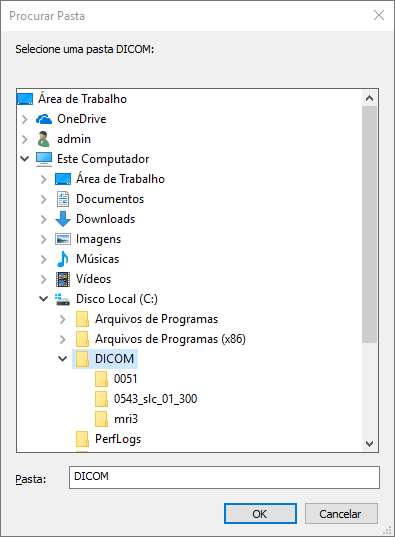
\includegraphics[scale=0.5]{../user_guide_figures/invesalius_screen/import_select_folder_pt.png}
\caption{Seleção de diretório}
\label{fig:win_folder}
\end{figure}

\hspace{.2cm}

Enquanto o InVesalius procura por arquivos DICOM no diretório, é exibido o progresso
do carregamento dos arquivos verificados, como ilustra a figura \ref{fig:ver_file}.

\begin{figure}[!htb]
\centering
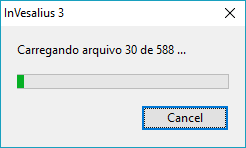
\includegraphics[scale=0.6]{../user_guide_figures/invesalius_screen/import_load_files_pt.png}
\caption{Status de verificação e carregamento de arquivos}
\label{fig:ver_file}
\end{figure}

\newpage

Se arquivos DICOM forem encontrados, é aberta uma janela (figura \ref{fig:win_import})
para selecionar o paciente e a respectiva série que se deseja abrir. Também é possível
pular imagens para reconstrução.

\begin{figure}[!htb]
\centering
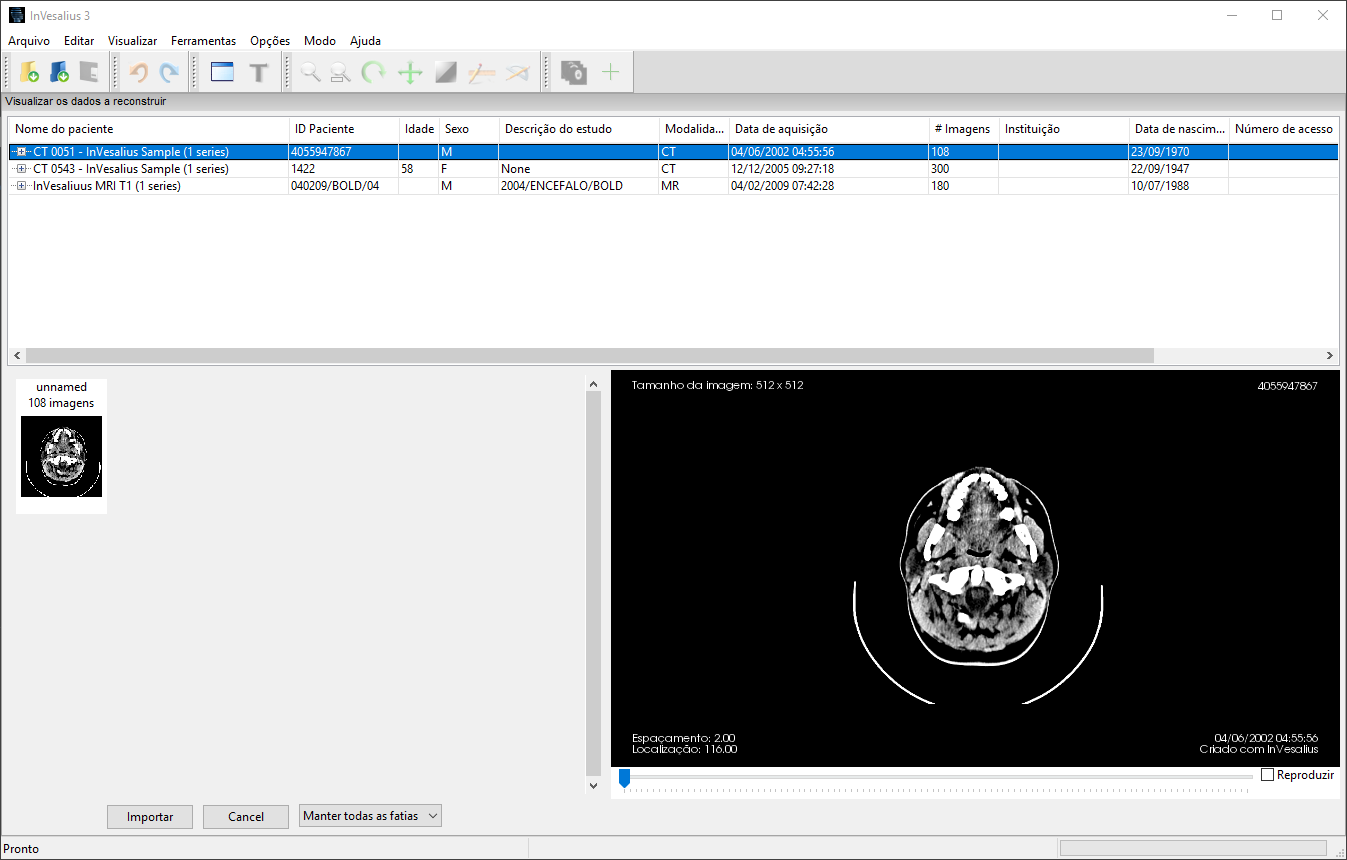
\includegraphics[scale=0.4]{../user_guide_figures/invesalius_screen/import_window_pt.png}
\caption{Tela de importação}
\label{fig:win_import}
\end{figure}

\newpage

Caso deseje importar uma série com todas as imagens presentes, clique em "\textbf{+}" ao
lado do nome do paciente para expandir as séries a ele pertencentes. Dê um \textbf{clique duplo}
com o botão \textbf{esquerdo} do mouse sobre a descrição da série. Veja a figura
\ref{fig:import_serie}.

\begin{figure}[!htb]
\centering
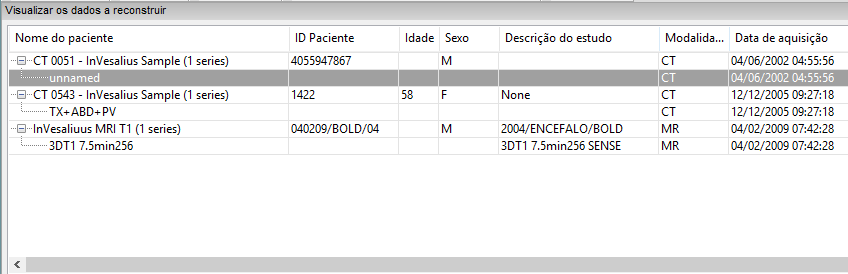
\includegraphics[scale=0.5]{../user_guide_figures/invesalius_screen/import_window_detail_pt.png}
\caption{Seleção de série}
\label{fig:import_serie}
\end{figure}
 
%\hspace{.2cm}

Em alguns casos, em particular quando não se dispõe de um computador com memória e/ou
processamento satisfatórios para trabalhar com muitas imagens em uma série, pode ser
recomendável pular (ignorar) algumas delas. Para isso, clique \textbf{uma vez} com o botão
\textbf{esquerdo} do mouse sobre a descrição da série (figura \ref{fig:import_serie}) e selecione
quantas imagens serão puladas (figura \ref{fig:skip_image}). Clique em \textbf{Importar}.

\begin{figure}[!htb]
\centering
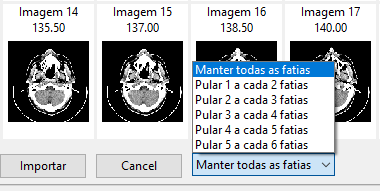
\includegraphics[scale=0.6]{../user_guide_figures/invesalius_screen/import_window_skip_slice_pt.png}
\caption{Pular imagens}
\label{fig:skip_image}
\end{figure}

%\hspace{.2cm}

Caso seja detectado quantidade insuficiente de memória disponível na hora de carregar as imagens é recomentado 
reduzir a resolução das fatias para trabalhar com visualização volumétrica e de superfície, como mostra a janela \ref{fig:resize_image}. 
As fatias serão redimensionadas de acordo com a porcentagem em relação a resolução original. Por exemplo, 
se cada fatia do exame contém a dimensão de 512 x 512 pixeis e for sugerido a "Porcentagem da resolução original" em 60\%, 
cada imagem resultante terá 307 x 307 pixeis. Caso deseje abrir com a resolução original selecione o valor 100.

\begin{figure}[!htb]
\centering
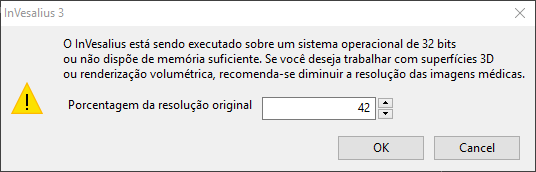
\includegraphics[scale=0.5]{../user_guide_figures/invesalius_screen/import_window_lower_memory_pt.png}
\caption{Redução de dimensão da imagem}
\label{fig:resize_image}
\end{figure}

Se a imagem foi obtida com o gantry inclinado, será necessário fazer a correção para evitar deformações na reconstrução. O InVesalius permite fazer essa correção. Ao importar uma imagem com o gantry inclinado aparecerá uma janela com o grau de inclinação do tilt (figura~\ref{fig:gantry_tilt}). É possível alterar esse valor, mas não é recomendável. Clique no botão \textbf{OK} para fazer a correção. Se clicar em \textbf{Cancelar} a reconstrução será realizada sem a correção.

\begin{figure}[!htb]
\centering
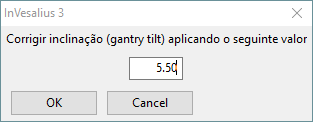
\includegraphics[scale=0.75]{../user_guide_figures/invesalius_screen/window_gantry_tilt_pt.png}
\caption{Correção de gantry tilt}
\label{fig:gantry_tilt}
\end{figure}

Após os procedimentos anteriores, será apresentada uma janela (figura \ref{fig:prog_recons}) com o progresso
da reconstrução (quando as imagens são empilhadas e interpoladas).

\begin{figure}[!htb]
\centering
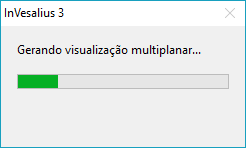
\includegraphics[scale=0.6]{../user_guide_figures/invesalius_screen/import_window_progress.png} 
\caption{Progresso da reconstrução}
\label{fig:prog_recons}
\end{figure}

\newpage

\section{Analyze}

Para importar arquivos no formato Analyze, no menu \textbf{Arquivo}, clique na opção \textbf{Importar outros arquivos...} em seguida a opção \textbf{Analyze} como mostra a figura \ref{fig:analyze_menu}.

\begin{figure}[!htb]
\centering
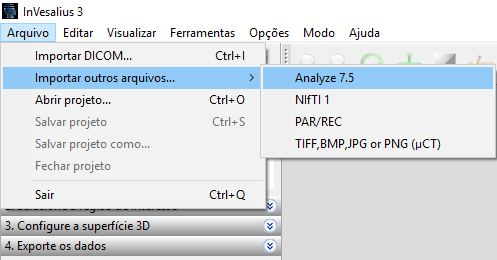
\includegraphics[scale=0.4]{../user_guide_figures/invesalius_screen/import_analyze_menu_pt.png}
\caption{Menu para importar imagens no formato analyze}
\label{fig:analyze_menu}
\end{figure}

Selecione o arquivo do tipo Analyze, na extensão \textbf{.hdr} e clique em \textbf{Abrir}. (figura \ref{fig:analyze_import}).

\begin{figure}[!htb]
\centering
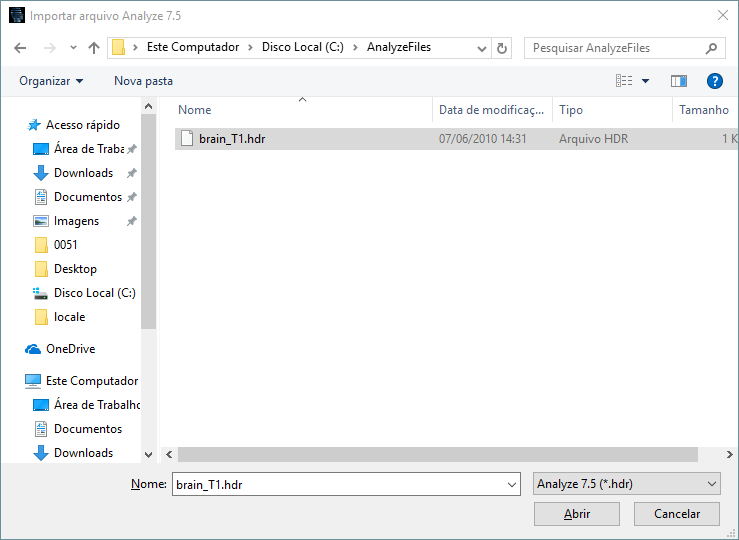
\includegraphics[scale=0.4]{../user_guide_figures/invesalius_screen/import_analyze_window_pt.png}
\caption{Importar imagens no formato analyze}
\label{fig:analyze_import}
\end{figure}

\section{NIfTI}

Para importar arquivos no formato NIfTI, no menu \textbf{Arquivo}, clique na opção \textbf{Importar outros arquivos...} em seguida a opção \textbf{NIfTI} como mostra a figura \ref{fig:import_nifti_menu_pt}.

\begin{figure}[!htb]
\centering
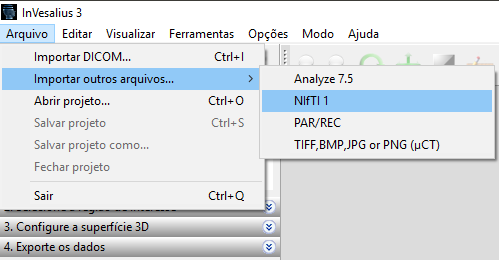
\includegraphics[scale=0.4]{../user_guide_figures/invesalius_screen/import_nifti_menu_pt.png}
\caption{Menu para importar imagens no formato NIfTI}
\label{fig:import_nifti_menu_pt}
\end{figure}

Selecione o arquivo do tipo NIfTI, na extensão \textbf{nii.gz} ou \textbf{.nii} e clique em \textbf{Abrir}. (figura \ref{fig:import_nifti_window_pt}). Caso o arquivo esteja em outra extensão como \textbf{.hdr}, selecione a opção \textbf{all files(*.*)}.

\begin{figure}[!htb]
\centering
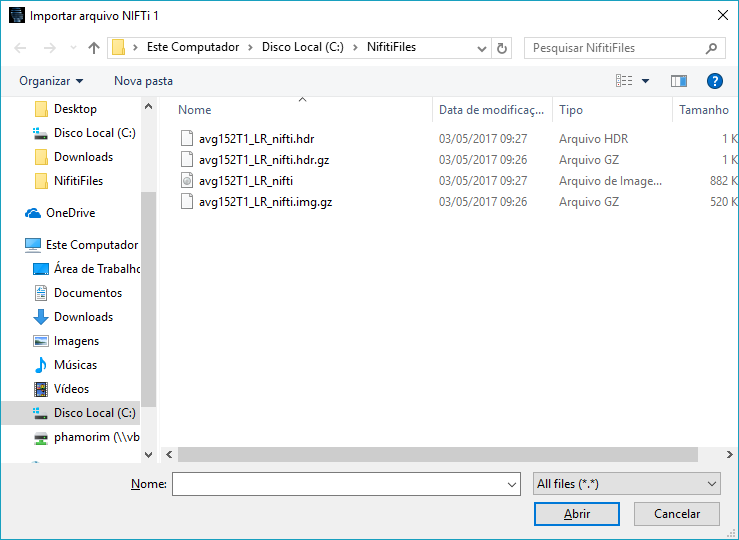
\includegraphics[scale=0.4]{../user_guide_figures/invesalius_screen/import_nifti_window_pt.png}
\caption{Importar imagens no formato NIfTI}
\label{fig:import_nifti_window_pt}
\end{figure}

\section{PAR/REC}


Para importar arquivos no formato PAR/REC, no menu \textbf{Arquivo}, clique na opção \textbf{Importar outros arquivos...} em seguida a opção \textbf{PAR/REC} como mostra a figura \ref{fig:import_parrec_menu_pt}.

\begin{figure}[!htb]
\centering
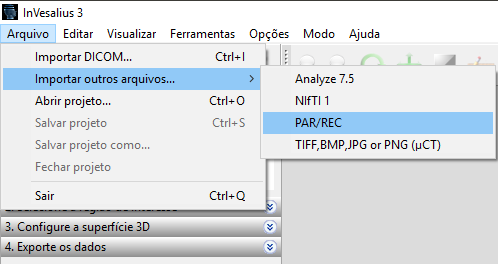
\includegraphics[scale=0.4]{../user_guide_figures/invesalius_screen/import_parrec_menu_pt.png}
\caption{Menu para importar imagens no formato PAR/REC}
\label{fig:import_parrec_menu_pt}
\end{figure}

Selecione o arquivo do tipo PAR/REC, na extensão \textbf{.par} e clique em \textbf{Abrir}. (figura \ref{fig:import_parrec_window_pt}). Caso o arquivo esteja sem extensão, selecione a opção \textbf{all files(*.*)}.

\begin{figure}[!htb]
\centering
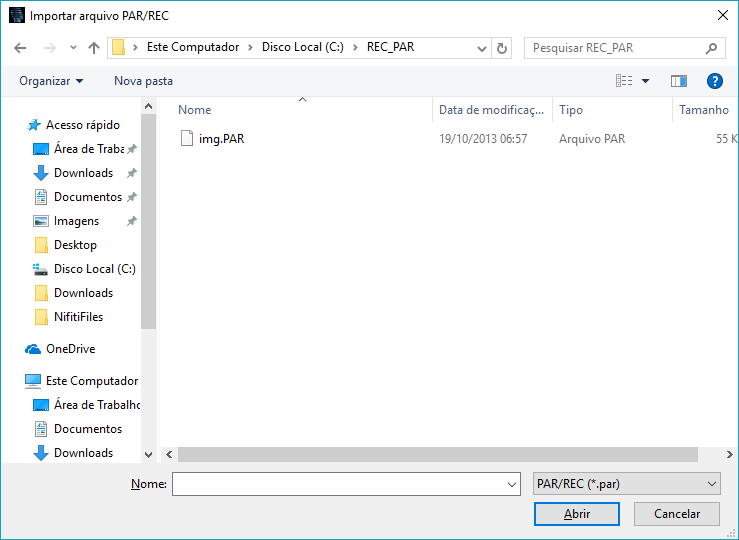
\includegraphics[scale=0.4]{../user_guide_figures/invesalius_screen/import_parrec_window_pt.png}
\caption{Importar imagens no formato PAR/REC}
\label{fig:import_parrec_window_pt}
\end{figure}



\section{TIFF, JPG, BMP, JPEG ou PNG (micro-CT)}

Arquivos em formato TIFF, JPG, BMP, JPEG ou PNG para reconstrução podem ser providos de equipamentos de microtomografia (micro-CT ou $\mu$CT) e outros. O InVesalius importa arquivos nesses formatos desde que os pixels presentes estejam em escala de cinza.

Para importar, clique no menu \textbf{Arquivo} e na opção \textbf{Importar outros arquivos...} em seguida clique na opção \textbf{TIFF, JPG, BMP, JPEG ou PNG ($\mu$CT)} como mostra a figura~\ref{fig:import_bmp_menu_pt}. 

\begin{figure}[!htb]
\centering
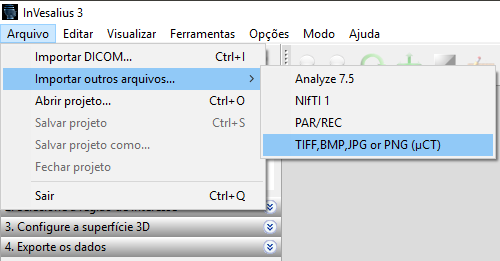
\includegraphics[scale=0.4]{../user_guide_figures/invesalius_screen/import_bmp_menu_pt.png}
\caption{Importar imagens no formato BMP e outros}
\label{fig:import_bmp_menu_pt}
\end{figure}

Selecione o diretório que contenha os arquivos, como mostra a figura \ref{fig:import_bmp_select_folder}. O InVesalius irá procurar por arquivos também em subdiretórios do diretório escolhido, caso existam.

Clique em \textbf{OK}.

\begin{figure}[!htb]
\centering
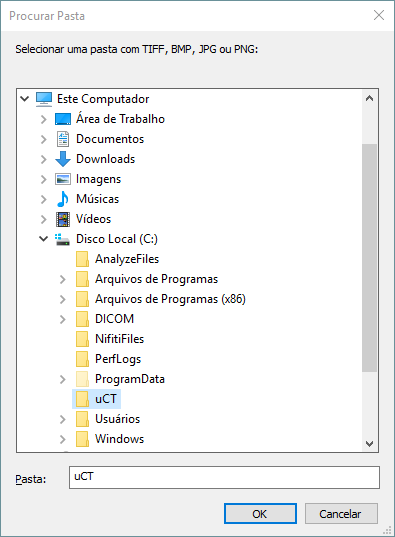
\includegraphics[scale=0.5]{../user_guide_figures/invesalius_screen/import_bmp_select_folder_pt.png}
\caption{Seleção de diretório}
\label{fig:import_bmp_select_folder}
\end{figure}


Enquanto o InVesalius procura por arquivos TIFF, JPG, BMP, JPEG ou PNG no diretório, é exibido o progresso do carregamento dos arquivos verificados, como ilustra a figura \ref{fig:import_bmp_load_pt}.

\begin{figure}[!htb]
\centering
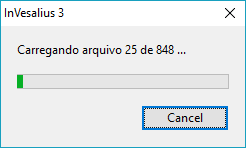
\includegraphics[scale=0.6]{../user_guide_figures/invesalius_screen/import_bmp_load_pt.png}
\caption{Status de verificação e carregamento de arquivos}
\label{fig:import_bmp_load_pt}
\end{figure}


Se arquivos do tipo TIFF, JPG, BMP, JPEG ou PNG  forem encontrados, é aberta uma janela (figura~\ref{fig:import_bmp_window_pt}) para exibir os arquivos encontrados elegíveis para reconstrução. Também é possível pular imagens para reconstrução ou remover arquivos da lista para reconstrução. Os arquivos são ordenados de acordo com o nome do arquivo, recomenda-se utilizar números em seus nomes de acordo com a ordem que deseja-se obter na reconstrução.

\begin{figure}[!htb]
\centering
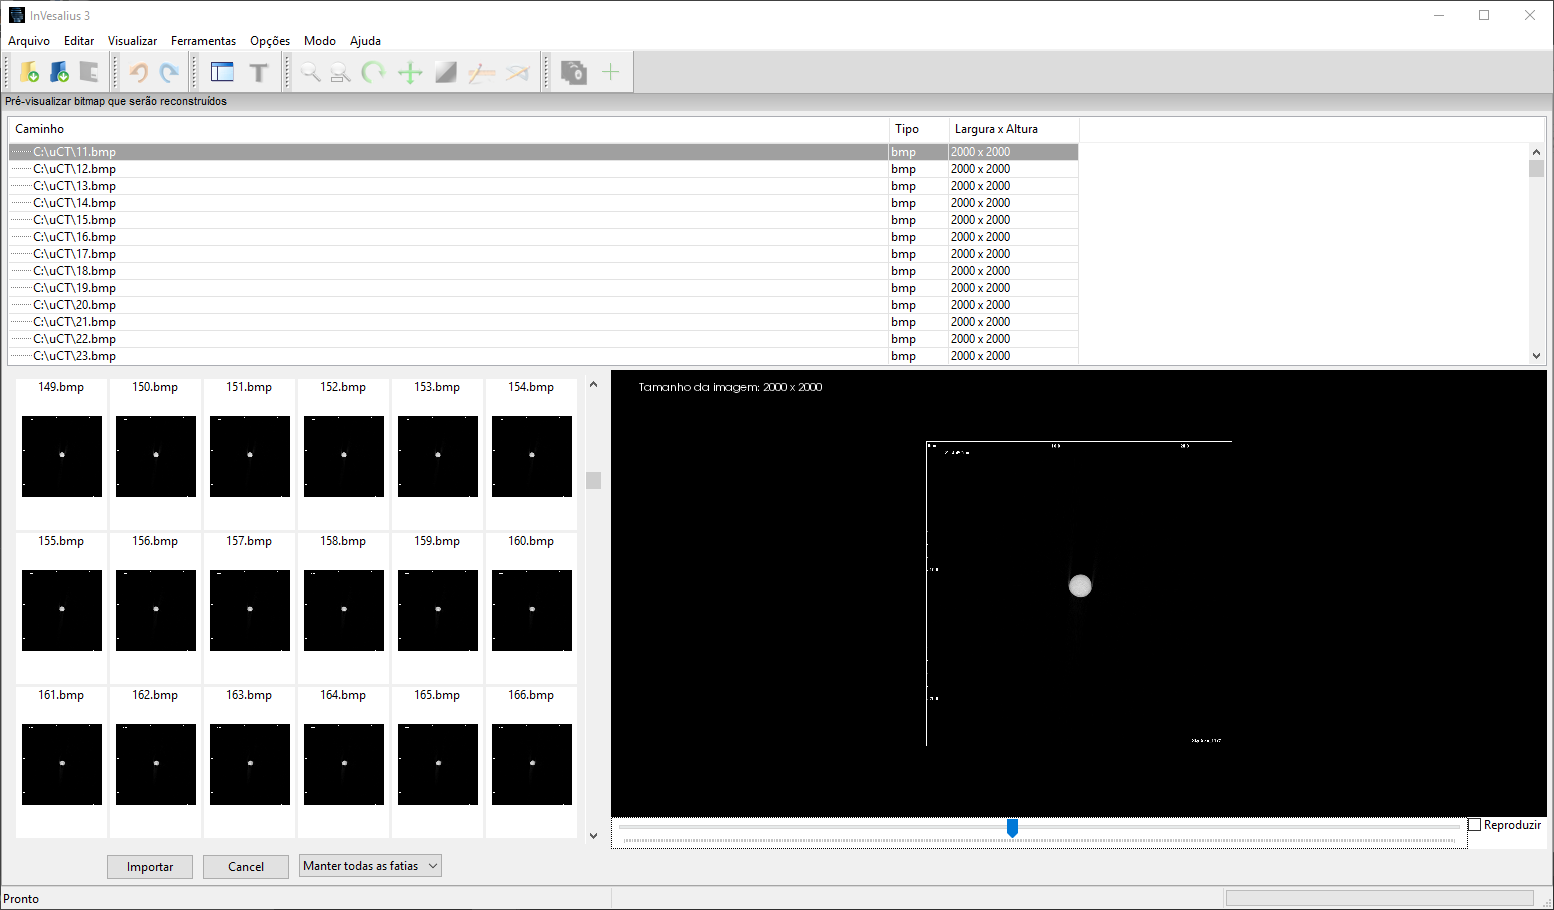
\includegraphics[scale=0.3]{../user_guide_figures/invesalius_screen/import_bmp_window_pt.png}
\caption{Janela para importação de arquivos do tipo BMP.}
\label{fig:import_bmp_window_pt}
\end{figure}

Para excluir os arquivos que não são de interesse, é possível selecionar um arquivo clicando com o \textbf{botão esquerdo do mouse} e em seguida pressionar a tecla \textbf{delete}. É possível também escolher uma faixa de arquivos para deletar, para isso é necessário clicar com o \textbf{botão esquerdo do mouse} no primeiro arquivo da faixa, manter pressionada a tecla \textbf{shift}, clicar novamente com o \textbf{botão esquerdo do mouse} no último arquivo da faixa e finalmente pressionar o botão \textbf{delete}.
 
A exemplo da importação de arquivos DICOM, é possível pular imagens BMP para reconstrução. Em alguns casos, em particular quando não se dispõe de um computador com memória e/ou processamento satisfatórios para trabalhar com muitas imagens em uma série, pode ser recomendável pular (ignorar) algumas delas. Para isso, selecione quantas imagens serão puladas (figura \ref{fig:import_bmp_skip_pt}). Clique em \textbf{Importar}.

\begin{figure}[!htb]
\centering
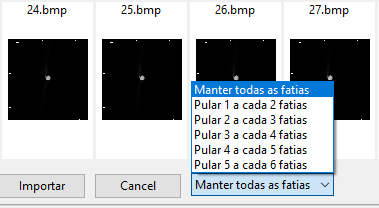
\includegraphics[scale=0.4]{../user_guide_figures/invesalius_screen/import_bmp_skip_pt.png}
\caption{Tela de importação}
\label{fig:import_bmp_skip_pt}
\end{figure}

Para a reconstrução desse tipo de arquivo é necessário definir um nome para o projeto, indicar qual a orientação das imagens (axial, coronal ou sagital), espaçamento do voxel ($X$, $Y$ e $Z$) em \textbf{milímetros} como mostra a figura~\ref{fig:import_bmp_spacing_pt}. O espaçamento do voxel em $X$ é largura do pixel de cada imagem, $Y$ o comprimento do pixel e $Z$ representa a distância de cada fatia (altura do voxel). 

Caso o conjunto de imagens seja de imagens de microtomografia, mais especificamente de equipamentos das marcas GE e Brucker, é possível que o InVesalius realize a leitura do arquivo texto com os parâmetros de aquisição que normalmente fica na mesma pasta das imagens e insira automaticamente o espaçamento. Essa constatação pode ser feita quando os valores de $X$, $Y$ e $Z$ são diferentes de "1.00000000", caso contrário é necessário digitar os valores dos respectivos espaçamento. 

\textbf{Atenção, o espaçamento é um parâmetro primordial para a correta dimensão dos objetos no software. Espaçamento incorreto irá fornecer medidas incorretas.}

Uma vez preenchido todos os parâmetros, basta clicar no botão \textbf{Ok}.

\begin{figure}[!htb]
\centering
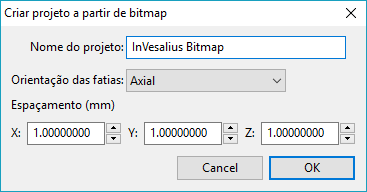
\includegraphics[scale=0.5]{../user_guide_figures/invesalius_screen/import_bmp_spacing_pt.png}
\caption{Tela de importação}
\label{fig:import_bmp_spacing_pt}
\end{figure}

Caso seja detectado quantidade insuficiente de memória disponível na hora de carregar as imagens é recomentado  reduzir a resolução das fatias para trabalhar com visualização volumétrica e de superfície, como mostra a janela \ref{fig:import_bmp_resize_pt}.  As fatias serão redimensionadas de acordo com a porcentagem em relação a resolução original. Por exemplo,  se cada fatia do exame contém a dimensão de 512 x 512 pixeis e for sugerido a "Porcentagem da resolução original" em 60\%, cada imagem resultante terá 307 x 307 pixeis. Caso deseje abrir com a resolução original selecione o valor 100.

\begin{figure}[!htb]
\centering
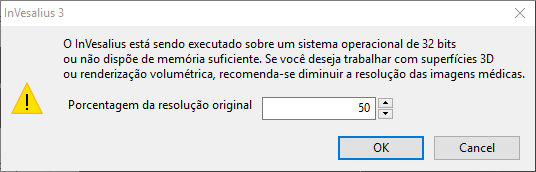
\includegraphics[scale=0.5]{../user_guide_figures/invesalius_screen/import_bmp_resize_pt.png}
\caption{Redimensionamento de imagens}
\label{fig:import_bmp_resize_pt}
\end{figure}


Após os passos anteriores é necessário aguardar um instante para completar a reconstrução multiplanar conforme mostra a figura~\ref{fig:import_bmp_mpr_pt.png}.

\begin{figure}[!htb]
\centering
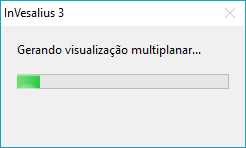
\includegraphics[scale=0.6]{../user_guide_figures/invesalius_screen/import_bmp_mpr_pt.png}
\caption{Reconstrução multiplanar em andamento.}
\label{fig:import_bmp_mpr_pt.png}
\end{figure}
